% Tikz File 'mytikz.tex'
\documentclass{standalone}
\usepackage{amsmath,xparse}
\DeclareMathOperator{\vsd}{VSD}
\DeclareMathOperator{\asd}{ASD}
\DeclareMathOperator{\ea}{EA}
\DeclareMathOperator{\bb}{BB}
\DeclareMathOperator{\voc}{VC}
\usepackage{tikz}

\pgfdeclarelayer{bg} 
\pgfdeclarelayer{background}
\pgfdeclarelayer{foreground}
\pgfsetlayers{background,main,foreground}
\tikzstyle{sensor}=[draw, text width=2em, 
    text centered, minimum height=2.5em]
 \tikzstyle{v} =[circle, thick, minimum size=0.8cm, draw=black]

\begin{document}
 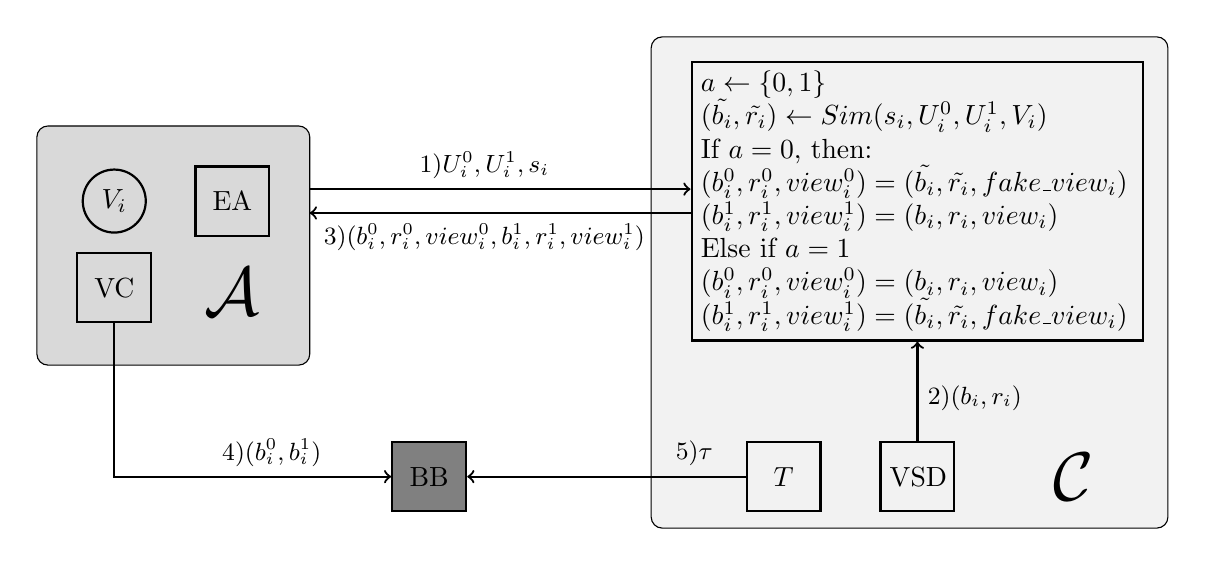
\begin{tikzpicture}[thick]
  \node[draw,rectangle]  at (-3.5, 5) (ea)[sensor] {$\ea$};
    \path (ea.south) +(-0,-0.7) node (a) {\Huge{$\mathcal{A}$}};
  \node[draw,rectangle,text width=5.5cm]  at (5.2, 5) (c) {$a \leftarrow \{0,1\} $ \\  $(\tilde{b_i}, \tilde{r_i}) \leftarrow Sim(s_i,U_i^0,U_i^1, V_i)$\\If $a=0$, then:\\ $(b_i^0, r_i^0,view_i^0) = (\tilde{b_i},\tilde{r_i},fake\_view_i)$\\ $(b_i^1,r_i^1,view_i^1)= (b_i,r_i,view_i)$ \\ Else if $a = 1$ \\$(b_i^0,r_i^0,view_i^0) = (b_i,r_i,view_i) $ \\$(b_i^1, r_i^1,view_i^1) = (\tilde{b_i},\tilde{r_i},fake\_view_i)$};
   \node[draw,rectangle]  at (5.2, 1.5) (vsd)[sensor] { $\vsd$};
   \node[draw,rectangle]  at (3.5, 1.5) (t)[sensor] { $T$};
      \node[draw,rectangle]  at (-5, 3.9) (vc)[sensor] { $\voc$};
         \node [ draw,circle] at (-5,5) (vfake)[v]{$V_i$};
      
           \node[draw,rectangle, fill = gray]  at (-1, 1.5) (bb)[sensor] { $\bb$};
   
   \draw[transform canvas={yshift=-1ex},->,shorten >=0.5cm] (c) node[font=\small, below,xshift=-5.5cm]  {$3) (b_i^0,r_i^0, view_i^0,b_i^1,r_i^1,view_i^1)$}  -- (ea);
      \draw[transform canvas={yshift=1ex},<-,shorten >=0.5cm] (c) node[font=\small, above,xshift=-5.5cm]  {$1) U_i^0,U_i^1,s_i$}  -- (ea);
   
   \draw[<-] (c) node[font=\small, right,yshift=-2.5cm,] {$2) (b_i,r_i)$} -- (vsd);
   
    \draw[<-] (bb) node[font=\small, right,xshift=3cm,yshift=0.3cm] {$5)\tau$} -- (t);
    
    \draw[<-] (bb) node[font=\small,above,xshift =-2cm] {$4) (b_i^0,b_i^1)$} -| (vc);
   
     \begin{pgfonlayer}{background}
        \path (vc.west |- ea.north)+(-0.5,0.5) node (e) {};
        \path (a.south -| ea.east)+(+0.5,-0.5) node (d) {};
        \path[rounded corners, draw=black, fill = gray!30]
            (e) rectangle (d);
    \end{pgfonlayer} 
    
     \begin{pgfonlayer}{background}
        \path (c.west |- c.north)+(-0.5,0.3) node (a) {};
        \path (vsd.south -| c.east)+(+0.3,-0.2) node (b) {};
        \path[rounded corners, draw=black, fill = gray!10]
            (a) rectangle (b);
    \end{pgfonlayer}
    \path (vsd.east) +(+1.5,0) node (RE) {\Huge{$\mathcal{C}$}};
  \end{tikzpicture}
\end{document}